\chapter{Results and Discussion}

\section{Introduction}
This chapter presents the results of the network resilience analysis by examining how seismic disruptions impact key transport network indicators. The findings are based on the betweenness centrality, beta index, gamma index, clustering coefficient, average degree, and redundancy indicator before and after disruption scenarios. By comparing these indicators, the chapter highlights how different road classifications and regional transport networks respond to disruptions, identifying the most vulnerable areas and critical links in Southern Italy.

The results are structured as follows: First, the general network indicators before and after disruption are presented, summarizing key trends and observations. Then, a detailed analysis of each indicator is provided, including percentage changes and their significance in assessing network resilience. The discussion focuses on identifying critical links and evaluating the degree of connectivity loss due to seismic events.

The first part of this analysis focuses on betweenness centrality, a key measure that identifies the most important road segments in facilitating movement across the transport network. The evaluation of critical road links before and after disruption provides insight into how seismic events redistribute traffic flow and increase congestion in alternative routes.

\section{Betweenness Centrality of Links Before and After Disruption}
Betweenness centrality is a fundamental measure in transport network analysis, representing the extent to which a link is used in the shortest paths across the network. Links with high betweenness centrality serve as major traffic conduits, meaning their failure would significantly impact regional connectivity. This section evaluates betweenness centrality before and after disruption, highlighting critical road links and the impact of seismic faults.

\subsection{Betweenness Centrality Before Disruption (Business-As-Usual Scenario)}

In the BAU scenario, the transport network operates without disruptions, meaning that betweenness centrality is distributed based on natural travel demand patterns and existing road capacities. The graphical representation of betweenness centrality in this scenario highlights the most important links for regional and interregional transport.

The network is classified into four categories based on betweenness centrality values:

\begin{itemize}
    \item \textbf{Red links (1.5\%)} are the most critical links, experiencing the highest level of centrality. These links are heavily concentrated around seismic faults 1 and 2, particularly in Campania, where primary road corridors support significant traffic flows.
    \item \textbf{Yellow links (10.5\%)} are high-importance links, mainly consisting of motorways and primary roads that provide essential long-distance connectivity.
    \item \textbf{Green links (35\%)} are moderately important routes, often serving as secondary alternatives to the primary road network.
    \item \textbf{Black links (53\%)} are the least critical, comprising rural, local, or low-traffic roads that contribute minimally to shortest-path flows.
\end{itemize}

The mean betweenness centrality in the BAU scenario is \textbf{0.0047}, with a standard deviation of \textbf{0.0020}, reflecting a network where a few highly centralized corridors dominate overall connectivity.

\subsection{Regional Differences in Betweenness Centrality Before Disruption}

The spatial distribution of high-centrality links varies significantly across different regions:

\textbf{Campania}, located in the western part of the study area, contains the highest concentration of red and yellow links, meaning that disruptions in this region would cause severe network fragmentation and increased travel times. This region serves as a key economic and transport hub, reinforcing the high reliance on major corridors.

\textbf{Puglia} exhibits a more balanced centrality distribution, with fewer red links and a greater proportion of yellow and green links. This indicates that Puglia’s network structure provides more redundancy and flexibility, making it moderately resilient to disruptions.

\textbf{Calabria}, particularly around Seismic Fault 3, has fewer high-centrality links, indicating that disruptions in this area would have a limited impact on overall network performance. The regional road network is less centralized, reducing the reliance on individual corridors.

These differences suggest that not all regions experience the same level of vulnerability, with Campania being the most critical, followed by Puglia, and Calabria being the least affected in a pre-disruption scenario.

\begin{figure}[H]
\centering
{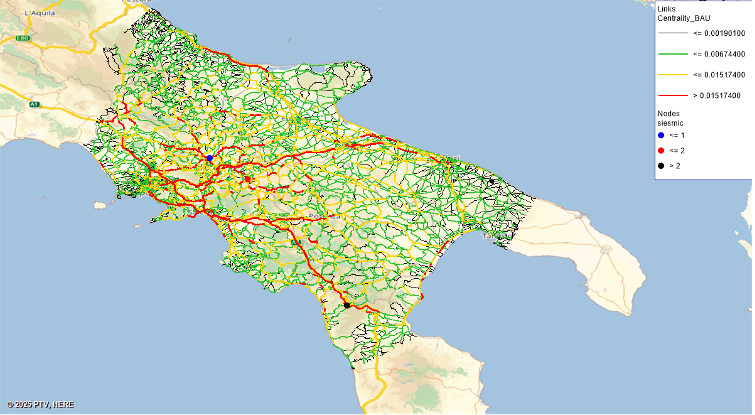
\includegraphics[width=1\textwidth]{images/Picture 1.png}}
    \caption{Betweenness Centrality of links ( BAU ) }
\end{figure}

\subsection{Changes in Betweenness Centrality After Disruption}
To assess how seismic events impact network connectivity, betweenness centrality was recalculated for six seismic fault scenarios. The analysis measures how critical link distributions change post-disruption and which road segments become more dominant in shortest-path calculations due to rerouting effects.

The table below summarizes the percentage change in the number of links classified as Red, Yellow, Green, and Black compared to the BAU scenario.

  \begin{table}[H]
\centering
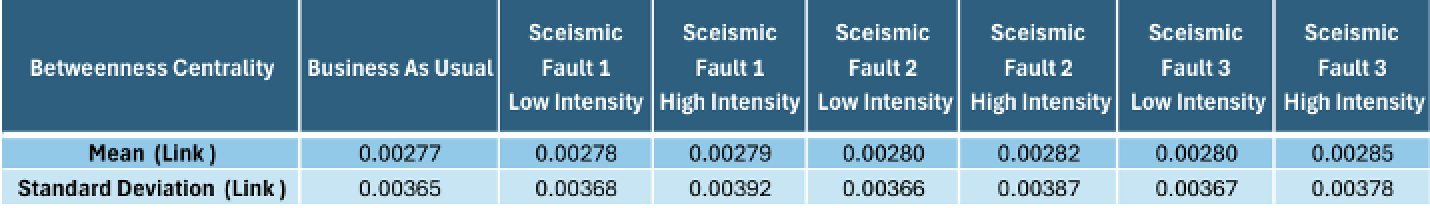
\includegraphics[width=\textwidth]{images/Table1.png}
\caption{Mean and Standard Deviation of Betweenness Centrality of Links}
\label{tab:betweenness_stats}
\end{table}

  \begin{table}[H]
\centering
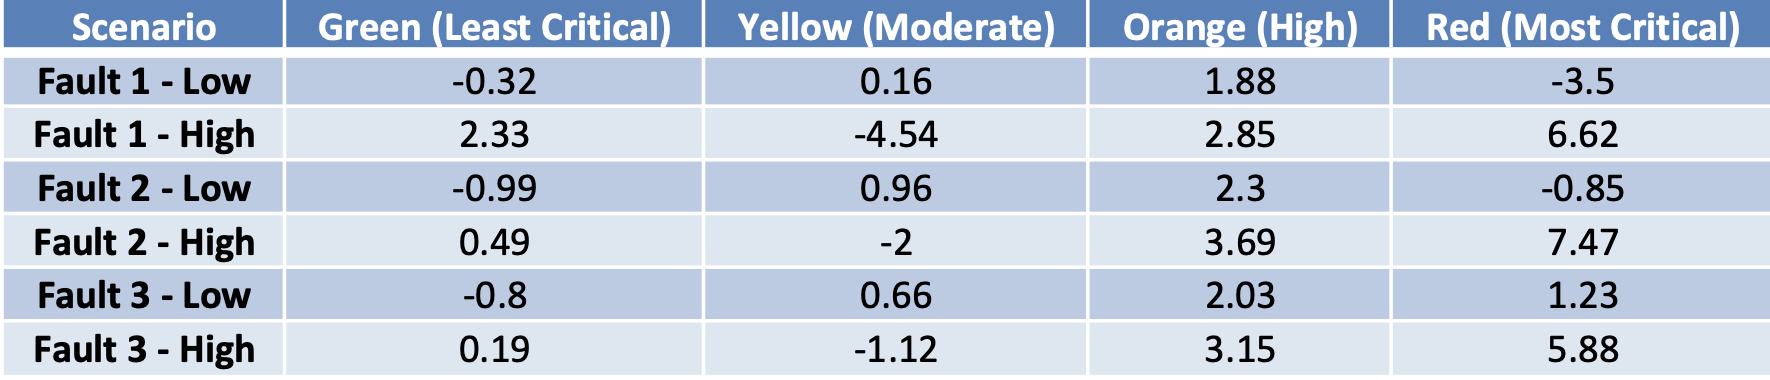
\includegraphics[width=\textwidth]{images/Table2.png}
\caption{Classification of Betweenness Centrality of Links}
\label{tab:classification_fault1}
\end{table}


The results indicate that Seismic 1 and 2 at the 15km buffer level cause the most severe shifts, with red links increasing by more than 6.5 percent, indicating new congestion points forming due to rerouted traffic. The greatest reductions in green links occur in Seismic 1 (15km) (2.33 percent), showing that some previously important secondary roads lost their significance after disruption.

Seismic Fault 3, particularly in the 15km scenario, sees a +5.88 percent increase in red links, meaning that some roads in Calabria gained importance, though not as significantly as in Campania. This suggests that while Calabria’s road network is generally less vulnerable, large-scale disruptions can still shift network reliance onto specific corridors.

These shifts in betweenness centrality confirm that primary roads (motorways and key interregional routes) become even more critical post-disruption, requiring strategic planning to mitigate congestion and maintain accessibility.

\subsection{Interpretation and Discussion of Results}
The betweenness centrality results reveal significant shifts in network criticality across different seismic scenarios. The analysis shows that the average betweenness centrality values decrease as seismic intensity increases, indicating that fewer links maintain high importance in shortest-path calculations post-disruption. The standard deviation values also decrease, suggesting that centrality values become more evenly distributed across the network, making it less centralized around key corridors.

The Business-As-Usual (BAU) scenario shows the highest average centrality at 0.00277, with a standard deviation of 0.00365, reflecting a network where a few highly centralized corridors dominate overall connectivity. As disruptions increase, centrality values decline, with the most significant drop occurring in Seismic 2 - High (0.00282 Mean, 0.00387 Std Dev), highlighting the severe impact of this disruption on network connectivity.

Campania remains the most vulnerable region, as it has the highest number of red and yellow links, meaning disruptions in this area cause widespread traffic shifts. Motorways continue to play a dominant role in connectivity, but seismic events increase reliance on secondary roads, which may not be designed to handle heavy rerouted traffic. Calabria remains relatively stable, reinforcing that its road network is less centralized and less dependent on a few critical links.

Seismic Fault 1 and Seismic Fault 2 create the highest impact, while Fault 3 disruptions are less significant. In large-scale disruptions (15km buffer), Seismic Fault 3 sees a noticeable increase in red links, suggesting that while Calabria is generally less vulnerable, major disruptions can still cause new bottlenecks to form.

By integrating these findings with the classification of links into Red, Yellow, Green, and Black, it becomes clear that seismic disruptions do not affect all roads equally. High-betweenness links are concentrated around Campania, confirming its importance as a key transport hub, while Calabria's dispersed network structure makes it more resilient in smaller-scale disruptions.

\subsection{Implications for Seismic Resilience and Conclusion}
The results highlight the need for targeted strategies to improve network resilience in earthquake-prone areas. Major motorways (yellow links) require reinforcement to prevent excessive strain on alternative routes when disruptions occur. The findings confirm that Campania is the most vulnerable region, requiring redundancy strategies such as alternative expressways and reinforced detour routes to ensure minimal disruptions.

The analysis also demonstrates that secondary roads(green links)fluctuate in importance post-disruption, meaning that alternative routing strategies should focus on preserving connectivity in high-betweenness areas near Fault 1 and Fault 2.

Betweenness centrality analysis provides a clear understanding of how the transport network adapts to seismic disruptions. By prioritizing the most affected areas, resilience strategies can be tailored to mitigate congestion, enhance redundancy, and ensure faster recovery after seismic events. These findings reinforce the importance of strengthening primary corridors and ensuring that secondary roads are adequately integrated into post-disruption traffic management plans.

\section{Node Betweenness Centrality Analysis}
Betweenness centrality for nodes provides insights into how crucial intersections and junctions are within the transport network. Nodes with high betweenness centrality act as critical connectors, facilitating traffic movement across the network. This section examines betweenness centrality in the Business-As-Usual (BAU) scenario and evaluates changes following seismic disruptions.

\subsection{Business-As-Usual (BAU) Scenario}
Before disruptions, node betweenness centrality was highest along motorways and trunk roads, particularly in \textbf{Campania (Fault 1)} and \textbf{Apulia (Fault 2)}. These regions serve as primary transport corridors, connecting urban and rural areas. The graphical representation of the Business-As-Usual (BAU) scenario indicates that:

\begin{itemize}
    \item \textbf{Most red nodes} (high centrality) are concentrated along major highways, motorways, and trunk roads.
    \item \textbf{Yellow and orange nodes} are found in secondary and tertiary roads, playing a supporting role in connectivity.
    \item \textbf{Green nodes}, which represent the lowest centrality values, dominate rural and less-connected areas.
\end{itemize}

The mean betweenness centrality for the BAU scenario was \textbf{0.004147}, with a standard deviation of \textbf{0.004700}, indicating a wide variability in node importance across the network.

\begin{figure}[H]
\centering
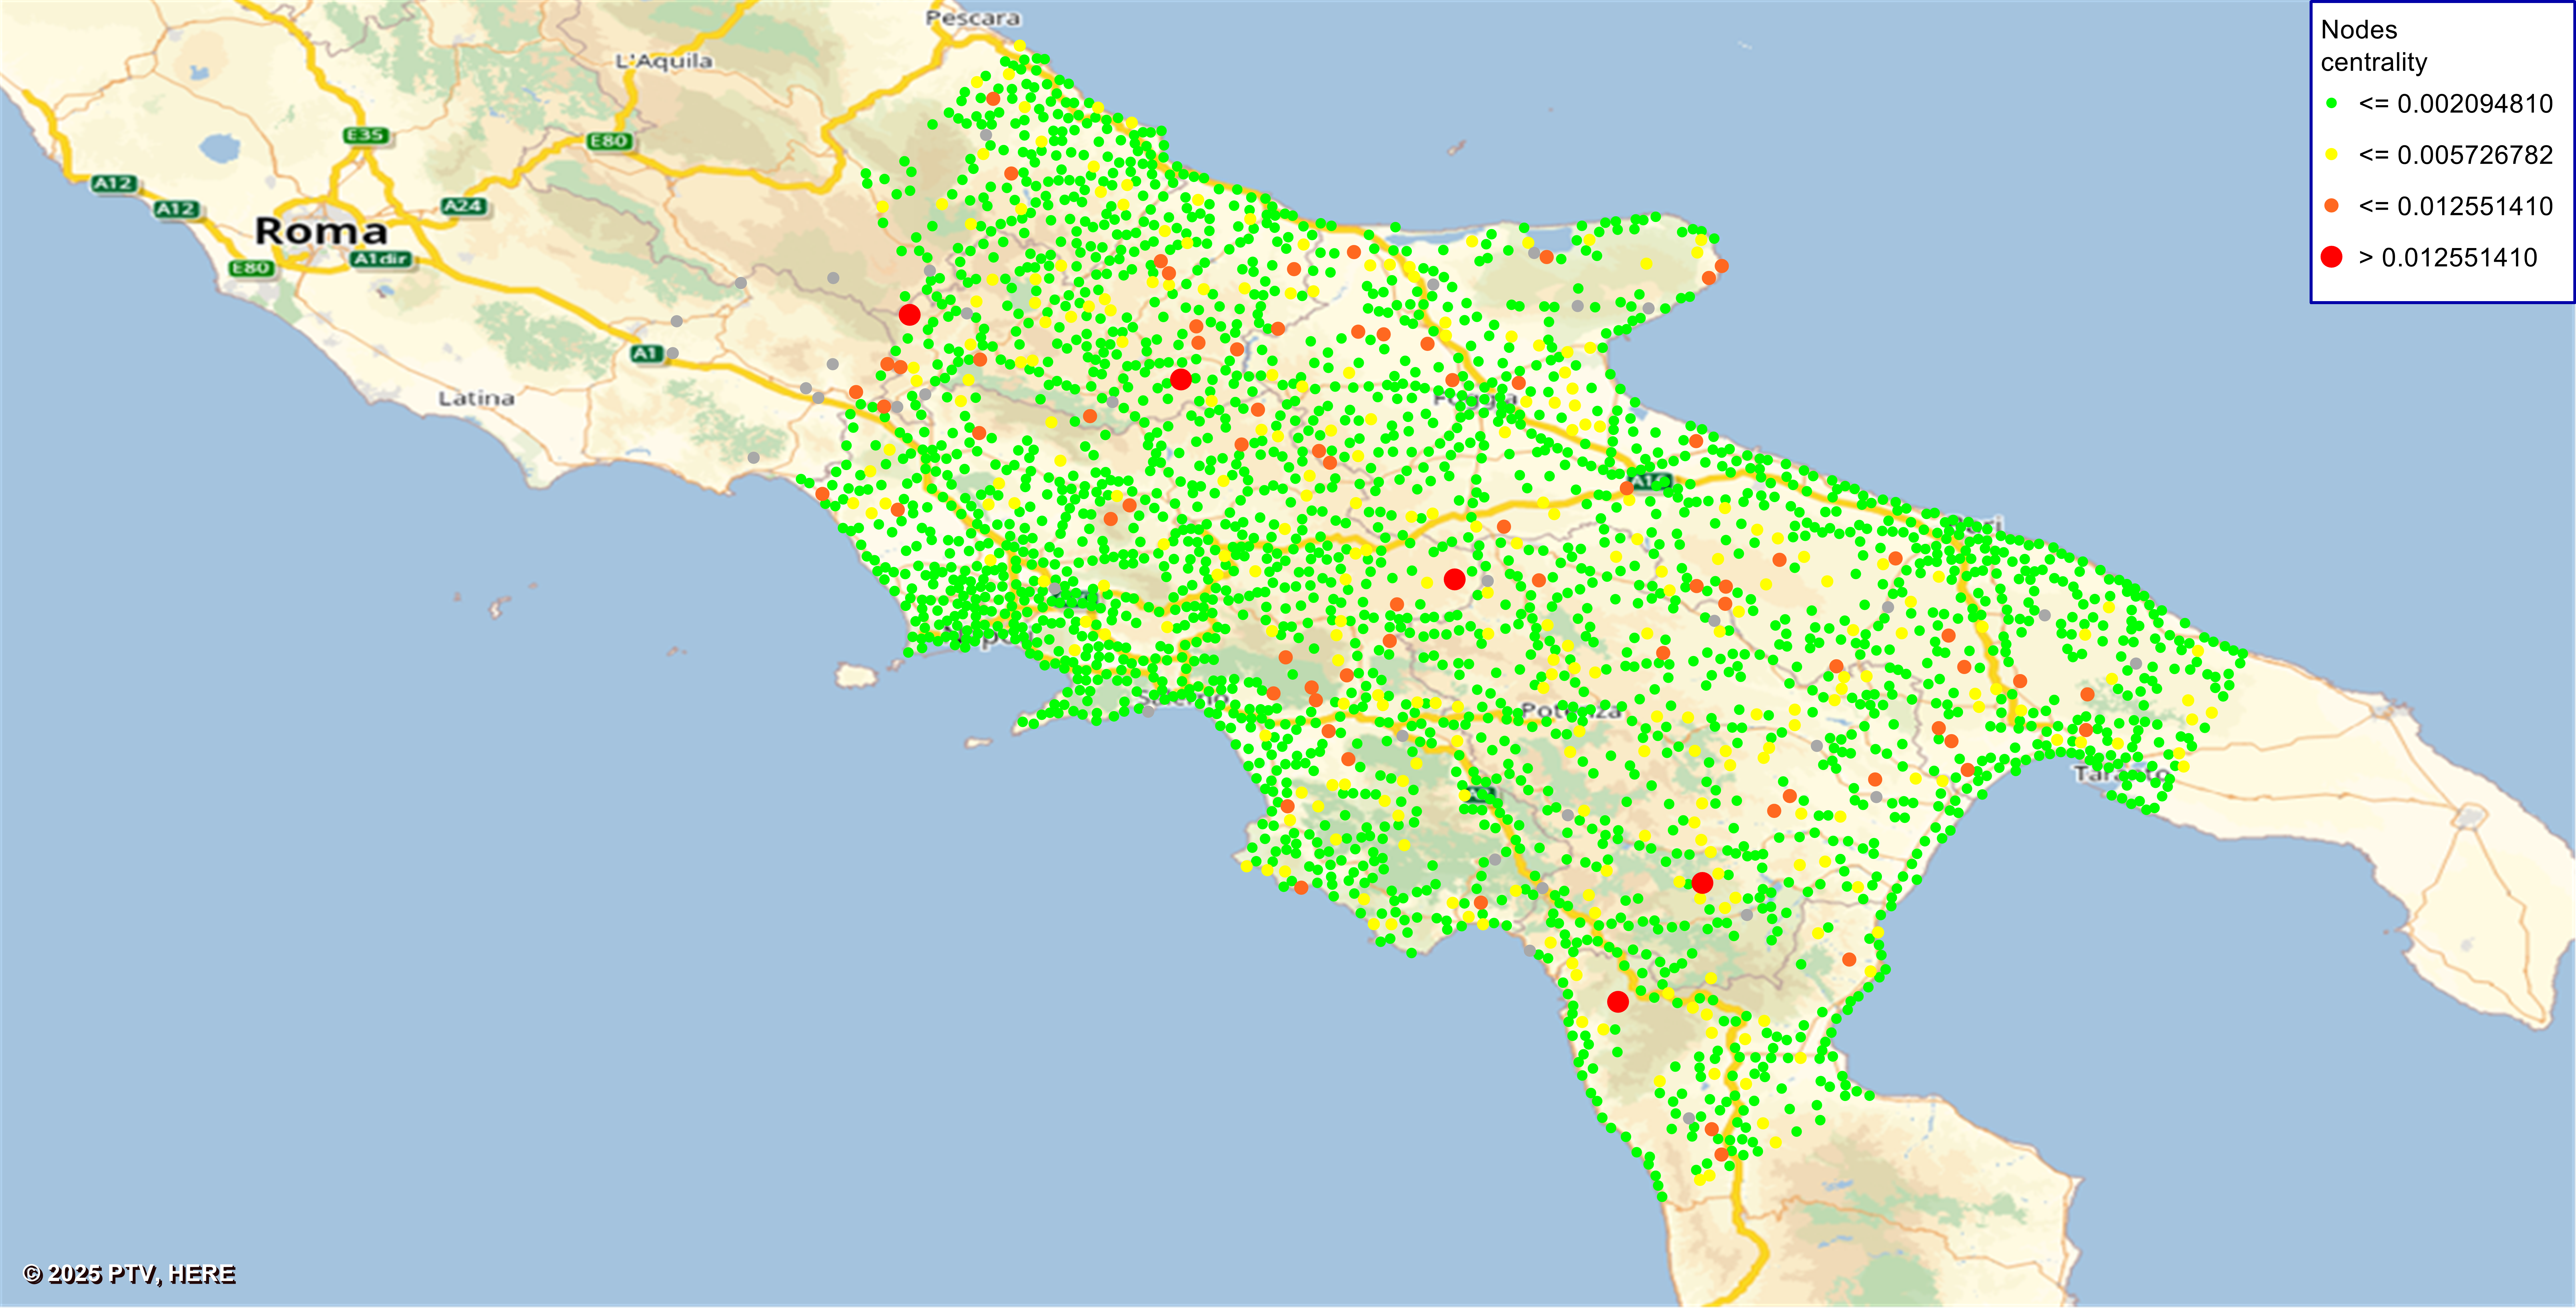
\includegraphics[width=1\textwidth]{images/Centrality_BAU_node 2.png}
\caption{Node Betweenness Centrality in BAU Scenario (Graphical Representation)}
\label{fig:bau_node_centrality}
\end{figure}


   \subsection{Changes in Betweenness Centrality After Disruption}
   After seismic disruptions, the mean and standard deviation of betweenness centrality shifted across all scenarios, reflecting the changes in network connectivity due to road failures.

 \begin{table}[H]
\centering
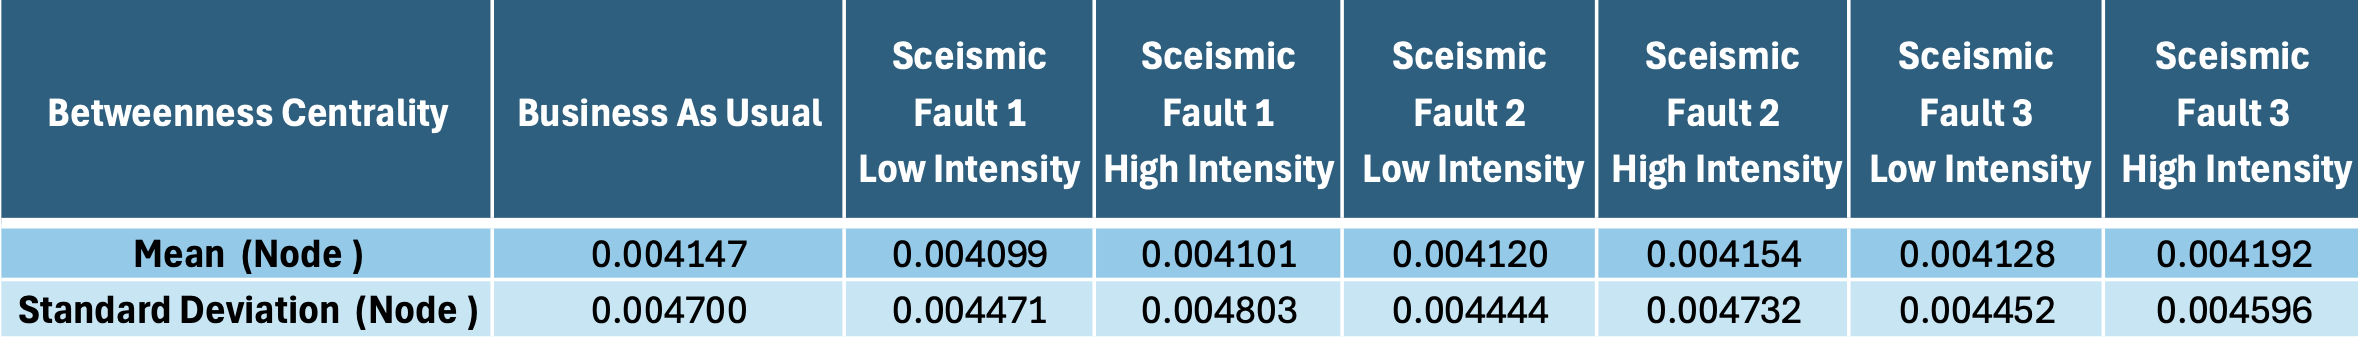
\includegraphics[width=1\textwidth]{images/Table3.png}
\caption{Mean and Standard Deviation of Node Betweenness Centrality Before and After Disruption.}
\label{tab:node_centrality_change}
\end{table}

\textbf{Key Observations}
\begin{itemize}
    \item Minor shifts in mean centrality indicate that the core network structure remains intact, but significant redistribution of centrality values occurs at a local level.
    \item \textbf{Seismic Fault 3 - High Intensity} had the highest mean increase (\textbf{0.004192}), indicating that critical nodes in Calabria became more central after disruption.
    \item Standard deviation increased in most high-intensity scenarios, signifying higher disparities in node importance, as some intersections gained significance while others lost connectivity.
\end{itemize}

 \begin{table}[H]
\centering
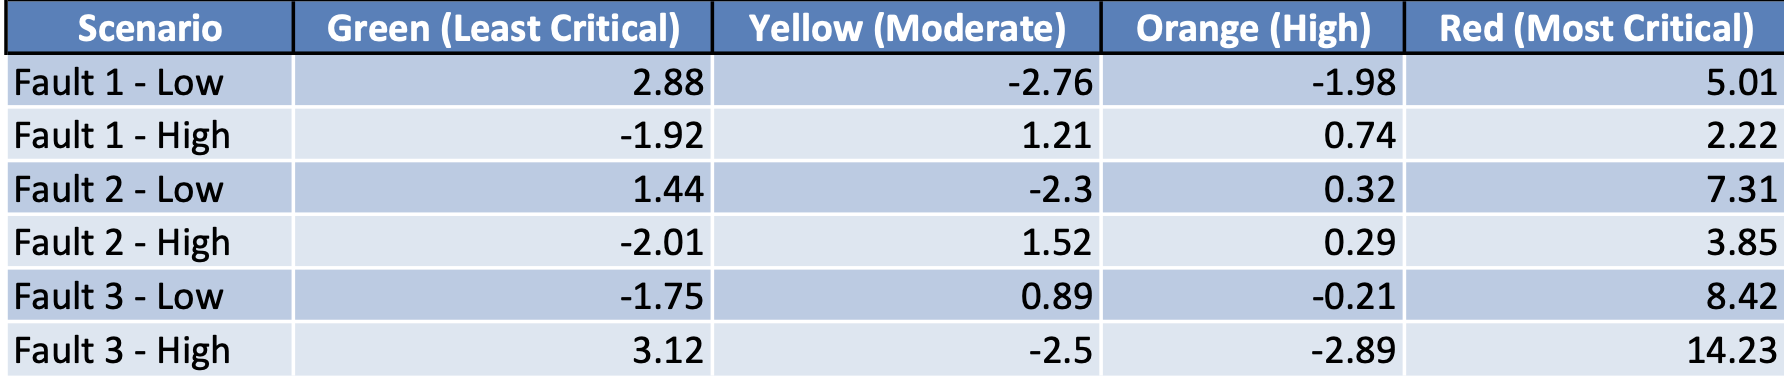
\includegraphics[width=1\textwidth]{images/Table4.png}
\caption{Percentage Change in Node Centrality Categories}
\label{tab:node_centrality_change_categories}
\end{table}

\subsection{Interpretation of Results}
\begin{itemize}
    \item \textbf{Fault 3 - High Intensity} produced the highest increase in red nodes (\textbf{+14.23\%}), significantly impacting network flow.
    \item \textbf{Fault 1} and \textbf{Fault 2} had lower but still notable increases in critical nodes, ranging between \textbf{+3.85\%} and \textbf{+7.31\%}.
    \item \textbf{Green (least critical)} nodes fluctuated across scenarios, but major shifts occurred in \textbf{red (most critical)} and \textbf{yellow (moderate)} nodes.
    \item \textbf{Yellow nodes} decreased in most scenarios, indicating that some moderately important nodes lost significance as traffic concentrated on a smaller set of high-betweenness intersections.
\end{itemize}

\subsection{Regional Differences and Seismic Fault 3’s Impact}
Although Fault 3 was initially the least critical area before the earthquake, it became the most affected after seismic events due to its lower number of nodes (intersections) and reduced network redundancy. This structural limitation made it highly vulnerable to disruptions, leading to the highest increase in critical nodes.

\textbf{Comparison Across Faults:}
\begin{itemize}
    \item \textbf{Fault 1 (Campania)} and \textbf{Fault 2 (Apulia)} had higher pre-disaster redundancy, distributing traffic shifts more evenly across the network.
    \item \textbf{Calabria (Fault 3)} had fewer alternative paths, making each disruption more impactful.
    \item \textbf{Seismic Fault 1} and \textbf{Fault 2} had smaller shifts in centrality values, reinforcing their robustness compared to Calabria.
\end{itemize}

\textbf{Implications for Seismic Resilience Planning:}
\begin{itemize}
    \item \textbf{Calabria} requires targeted infrastructure investments to enhance redundancy.
    \item \textbf{Traffic management strategies} should prioritize maintaining alternative routes in regions with fewer intersections.
    \item \textbf{Betweenness centrality shifts} indicate that post-earthquake detour planning must account for regions where minor disruptions cause large-scale bottlenecks.
\end{itemize}

\textbf{Final Takeaway}

Betweenness centrality analysis demonstrates that seismic events not only create new critical nodes but also significantly reshape the network hierarchy. While Campania and Apulia remained major transport corridors before and after seismic disruptions, Calabria's role changed significantly, evolving from a low-impact region to the most vulnerable in high-intensity scenarios. These findings highlight the necessity of pre-disaster planning to reinforce transport networks in low-density regions and ensure long-term resilience.

\section{Beta Index Analysis}
\subsection{Beta Index Before Disruption (BAU)}
The beta index measures network complexity by quantifying the ratio of links to nodes in the transport network. A higher beta index indicates a more interconnected and resilient network, while a lower beta index suggests a sparser network with fewer available alternative routes.

In the Business-As-Usual (BAU) scenario, the beta index is 1.4676, indicating a well-connected network with sufficient link redundancy. This suggests that under normal conditions, the transport network in Southern Italy provides multiple pathways for connectivity.

\subsection{Beta Index Changes After Disruption}
Following seismic disruptions, the beta index experienced minor variations across different earthquake scenarios. The table below summarizes the beta index values before and after disruptions, along with the percentage changes:

\begin{table}[H]
\centering
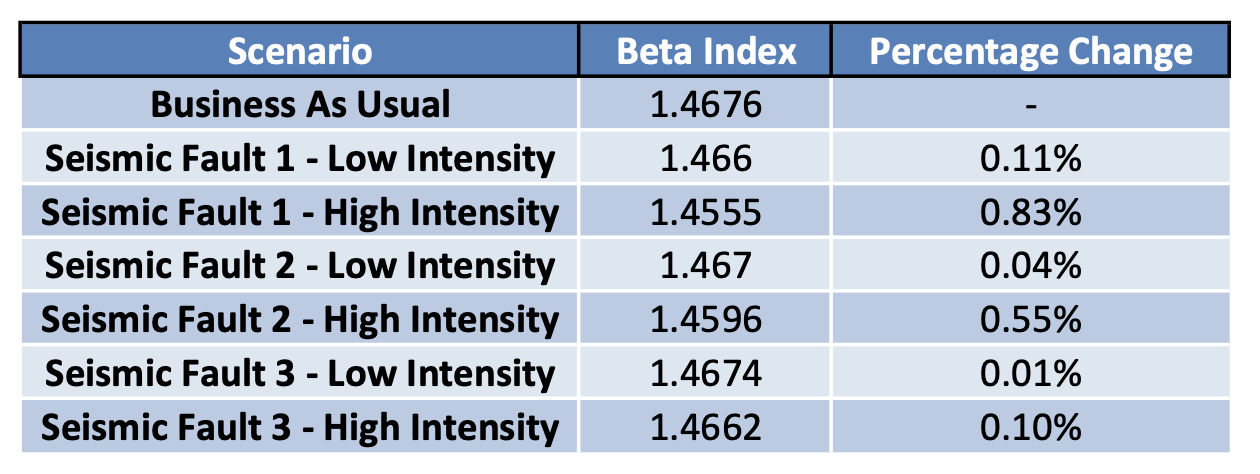
\includegraphics[width=1\textwidth]{images/Table5.png}
\caption{Beta Index Values and Percentage Change Across Seismic Disruption Scenarios}
\label{tab:beta_index_change}
\end{table}

The most significant drop in beta index occurred in Seismic Fault 1 - High Intensity (-0.83\%), indicating that this region experienced the greatest network fragmentation. This decline suggests a reduction in alternative routes due to road failures. Similarly, Seismic Fault 2 - High Intensity (-0.55\%) also exhibited a notable decrease, highlighting disruptions in this region.

Conversely, the Seismic Fault 3 scenarios showed minimal reductions in beta index (-0.01\% to -0.10\%), reinforcing that this region was initially less connected and therefore experienced fewer changes in network complexity.

\subsection{Interpretation of Results}
Seismic Fault 1 experienced the highest decrease in beta index, reflecting a greater disruption impact in this region. Seismic Fault 2 also showed a noticeable decline, indicating significant disruptions but with slightly better connectivity retention than Fault 1. Seismic Fault 3 remained relatively stable, suggesting that this region had fewer alternative links to begin with, making its overall network complexity less affected. Although all scenarios experienced some reduction in the beta index, the changes were minor, indicating that despite disruptions, the transport network maintains a reasonable level of connectivity.

\subsection{Implications for Seismic Resilience}
Regions with higher beta index reductions, such as Fault 1 and Fault 2, need targeted interventions like road reinforcements and redundancy planning. Alternative route planning should focus on areas where connectivity dropped the most, ensuring continued mobility after seismic events. Minimal beta index changes in Fault 3 indicate a pre-existing sparsity in the network, requiring long-term infrastructure planning rather than short-term resilience strategies.

This analysis provides a foundational understanding of how seismic events impact overall network complexity and highlights the importance of designing resilient road infrastructures that minimize connectivity losses.

\section{Gamma Index (Planar Coefficient) Analysis}
\subsection{Planar Coefficient Before Disruption (BAU)}
The gamma index (planar coefficient) measures the degree of connectivity within a transport network, specifically in planar networks such as road systems, where links are constrained by geographical and physical layout restrictions. A higher gamma index indicates a well-connected network with multiple route options, while a lower gamma index suggests a more fragmented or sparse network.

In the Business-As-Usual (BAU) scenario, the planar coefficient is 0.4892, suggesting that the Southern Italy transport network has a moderate level of connectivity, with some redundancy in routes but also certain constraints that limit the overall connectivity potential.

\subsection{Changes in Planar Coefficient After Disruption}
Seismic events impact the gamma index by disrupting road links, reducing the number of possible connections, and forcing traffic onto fewer alternative paths. The table below summarizes the planar coefficient before and after seismic disruptions, along with the percentage change for each scenario.

\begin{table}[H]
\centering
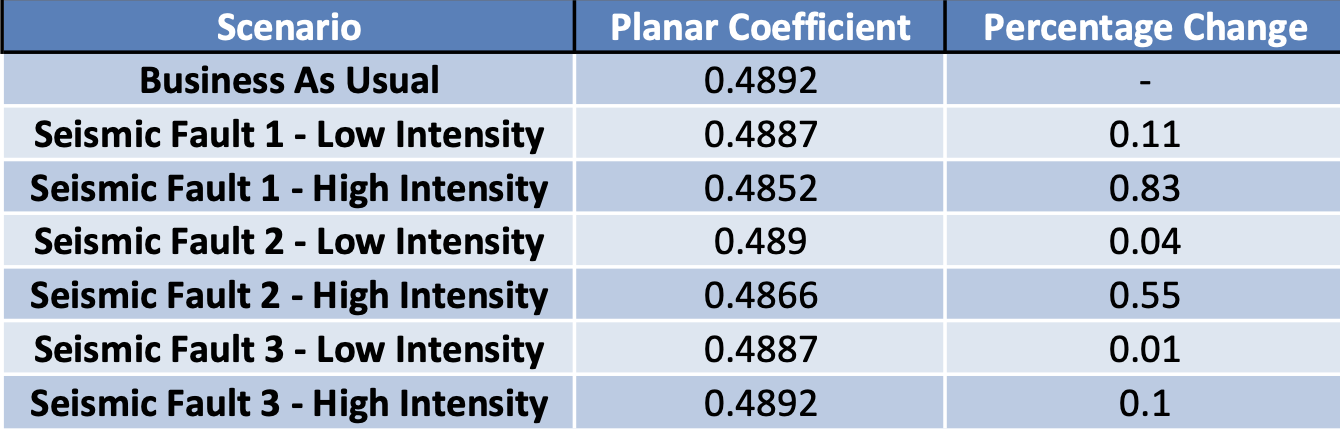
\includegraphics[width=1\textwidth]{images/Table6.png}
\caption{Planar Coefficient Values and Percentage Change Across Seismic Scenarios}
\label{tab:planar_coefficient_change}
\end{table}

The most significant drop in the gamma index occurred in Seismic Fault 1 - High Intensity (-0.83\%), indicating that this scenario caused the greatest disruption in connectivity. This reduction suggests that a higher number of links were lost or became non-functional, leading to a reduction in network-wide accessibility.

Seismic Fault 2 - High Intensity also exhibited a noticeable decrease of -0.55\%, confirming that this region also experienced significant connectivity disruptions. In contrast, Seismic Fault 3 scenarios showed minimal reductions (-0.01\% to -0.10\%), suggesting that the initial network configuration in this region was already sparse, and disruptions had a lower relative impact.

\subsection{Interpretation of Results}
Seismic Fault 1 experienced the highest reduction in gamma index, which means the region suffered from the greatest connectivity loss. Seismic Fault 2 showed a moderate drop, indicating that although the network faced disruptions, some level of connectivity was retained. Seismic Fault 3 experienced the smallest changes, reinforcing that its pre-existing sparse network did not experience significant additional fragmentation.

Despite disruptions across all scenarios, the changes in the gamma index remained relatively small, indicating that while local connectivity may have been affected, the overall network structure remained relatively intact. This suggests that while alternative routes were disrupted, the network was still able to maintain some level of redundancy.

\subsection{Implications for Seismic Resilience}
Regions with higher gamma index reductions, such as Fault 1 and Fault 2, require strategic interventions to reinforce network connectivity. This includes strengthening key road links, improving redundancy by adding new routes, and ensuring that critical road connections remain functional post-disruption.

In Fault 3, where the gamma index remained relatively stable, the focus should be on long-term infrastructure planning to improve baseline network connectivity rather than short-term mitigation. Since this region has a low-density network, seismic resilience strategies should aim to introduce new links and intersections to increase accessibility.

The gamma index analysis provides valuable insights into how seismic disruptions affect network-wide connectivity, highlighting the importance of reinforcing road infrastructures to minimize losses and ensure efficient transport flow in the aftermath of an earthquake.

\section{Clustering Coefficient (CC) Analysis}
\subsection{Clustering Coefficient Before Disruption (BAU)}
The clustering coefficient (CC) measures the extent to which nodes in a transport network tend to form local clusters. A higher clustering coefficient indicates a more locally connected and resilient network, while a lower value suggests a more fragmented network structure where nodes are less interconnected at a local level.

In the Business-As-Usual (BAU) scenario, the clustering coefficient is 0.8989, indicating a high level of local connectivity in the transport network of Southern Italy. This suggests that many nodes are well connected to their neighboring nodes, providing redundancy and alternative routes for local movements.

\subsection{Changes in Clustering Coefficient After Disruption}
Seismic events impact the clustering coefficient by disrupting links between nodes, potentially reducing the number of connections and increasing fragmentation in the network. The table below summarizes the clustering coefficient values before and after disruptions along with the percentage change for each scenario.

 \begin{table}[H]
\centering
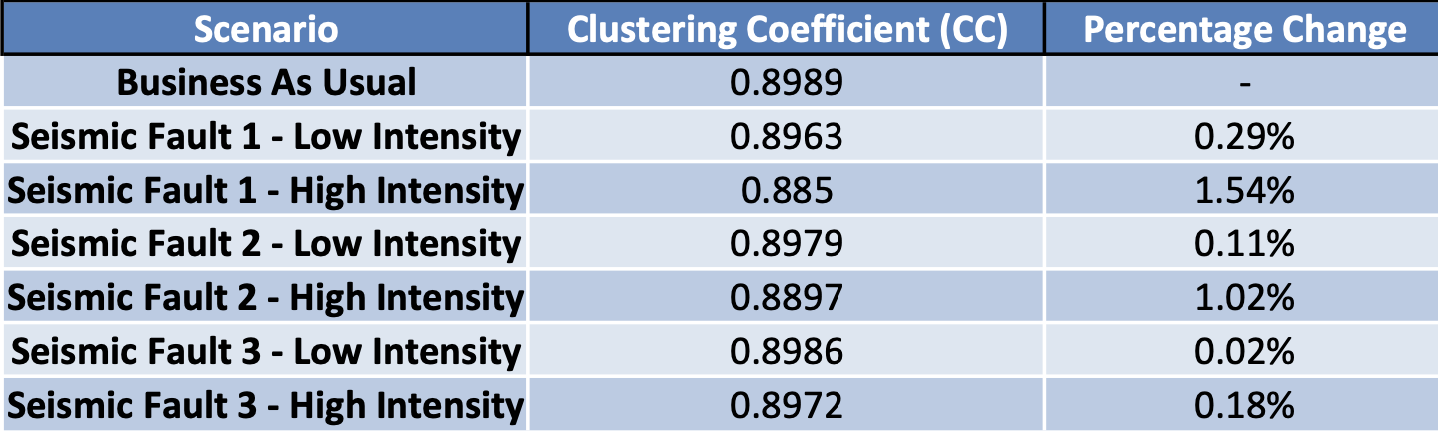
\includegraphics[width=1\textwidth]{images/Table7.png}
\caption{Clustering Coefficient Values and Percentage Change Across Seismic Scenarios}
\label{tab:clustering_coefficient_change}
\end{table}


The clustering coefficient slightly increases in all seismic scenarios, with the highest increase occurring in Seismic Fault 1 - High Intensity (1.54\%). This suggests that after disruptions, some nodes become more clustered as network pathways are restructured to maintain connectivity.

Seismic Fault 2 - High Intensity also shows a notable increase of 1.02\%, confirming that disruptions in this region led to increased local connectivity among surviving nodes. Conversely, Seismic Fault 3 scenarios exhibit the smallest changes (0.02\% to 0.18\%), reinforcing that this region’s network was less affected in terms of local clustering.

\subsection{Interpretation of Results}
The increase in the clustering coefficient across all scenarios suggests that seismic disruptions caused a redistribution of connectivity within local node groups. Instead of an overall loss in connectivity, the transport network adapted by forming denser clusters among remaining functional nodes, maintaining local accessibility despite disruptions.

Seismic Fault 1 had the highest increase in clustering coefficient, indicating that the affected region experienced greater traffic rerouting through local roads, reinforcing connectivity within smaller clusters. Seismic Fault 2 also showed significant clustering effects, but to a lesser extent. Seismic Fault 3 remained largely unchanged, suggesting that this region’s network structure was already optimized for local connectivity.

Despite disruptions, the increase in clustering coefficients indicates that the transport network retains local resilience, ensuring that nearby nodes continue functioning as effective clusters even when certain roads fail.

\subsection{Implications for Seismic Resilience}
The increase in clustering coefficients highlights the importance of local road networks in maintaining accessibility after seismic disruptions. Regions with high clustering coefficient increases, such as Fault 1 and Fault 2, require careful traffic management strategies to prevent congestion in local areas where traffic is redirected.

Since Fault 3 had minimal changes, long-term resilience planning should focus on improving overall connectivity rather than enhancing clustering. Future infrastructure development should consider reinforcing key road segments that link separate clusters, ensuring that local redundancy is maintained while also enhancing regional connectivity.

The clustering coefficient analysis provides insights into how local road networks adapt to disruptions, reinforcing the importance of well-connected node groups in maintaining regional mobility after an earthquake.

\section{Average Degree (CD) Analysis}
\subsection{Average Degree Before Disruption (BAU)}
The average degree (CD) quantifies network connectivity by measuring the average number of links per node. A higher CD value indicates a well-connected network with multiple alternative routes, while a lower CD value suggests a more fragmented network where nodes have fewer connections.

In the Business-As-Usual (BAU) scenario, the average degree is 2.966, indicating that nodes have an average of nearly three connections. This suggests that the transport network in Southern Italy has a relatively well-distributed connectivity structure, ensuring that most nodes maintain access to multiple routes.

\subsection{Changes in Average Degree After Disruption}
Seismic disruptions impact the average degree by reducing the number of functional links, thereby lowering the number of connections per node. The table below summarizes the average degree values before and after disruptions and their percentage change for each scenario.

\begin{table}[H]
\centering
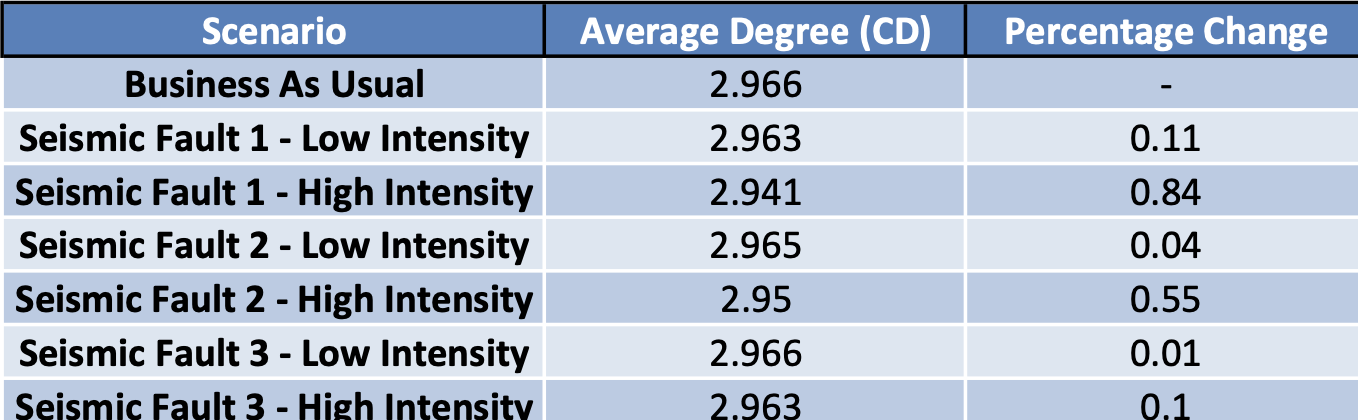
\includegraphics[width=1\textwidth]{images/Table8.png}
\caption{Average Degree Values and Percentage Change Across Seismic Scenarios}
\label{tab:average_degree_change}
\end{table}

The largest drop in average degree occurs in Seismic Fault 1 - High Intensity (0.84\%), indicating that this scenario resulted in the most significant reduction in connectivity. Seismic Fault 2 - High Intensity (0.55\%) also exhibits a noticeable decline, while Seismic Fault 3 scenarios show minimal reductions (0.01\% to 0.10\%), reinforcing that this region was already less connected and, therefore, less affected by disruptions.

\subsection{Interpretation of Results}
Seismic Fault 1 experienced the highest reduction in average degree, reflecting the largest impact on node connectivity. Seismic Fault 2 also showed a moderate decline, suggesting that while this region experienced disruptions, connectivity loss was not as severe as in Fault 1. Seismic Fault 3 remained relatively stable, with only minor changes in connectivity, indicating that its network was already sparse, and disruptions did not significantly alter its structure.

Despite connectivity losses across all scenarios, the percentage changes in average degree remained small, confirming that the transport network still retained some level of redundancy, preventing widespread disconnection.

\subsection{Implications for Seismic Resilience}
Regions with higher reductions in average degree, particularly Fault 1 and Fault 2, require targeted interventions to reinforce network connectivity. Strategies such as adding new links to critical nodes and ensuring that remaining routes can handle detoured traffic are essential for maintaining mobility after an earthquake.

Since Fault 3 had minimal reductions, long-term resilience planning should focus on improving overall connectivity rather than mitigating short-term disruptions. This region’s network needs additional links to increase redundancy, ensuring that future disruptions do not result in complete isolation of affected areas.

The average degree analysis provides valuable insights into how seismic disruptions impact network-wide connectivity, highlighting the importance of reinforcing key road connections to minimize transport system failures after an earthquake.

\section{Redundancy Analysis of the Transport Network Under Seismic Scenarios}
\subsection{Introduction to Redundancy Analysis}
Redundancy in transport networks refers to the system’s ability to maintain connectivity by providing alternative routes when primary roads fail. It is calculated as the ratio of travel time before disruption to travel time after disruption. A redundancy value close to 1 indicates a resilient network with minimal impact on travel time, whereas values approaching 0 signify severe disruptions, leading to complete disconnections.

The graphical representations categorize the zones based on their redundancy levels:

\begin{itemize}
    \item \textbf{Red zones}: These areas have a redundancy value of 0.000, indicating they are completely disconnected after disruption.
    \item \textbf{Blue zones}: These areas have a redundancy value of less than 0.900, meaning they experience increased travel times but remain accessible.
\end{itemize}

This section evaluates how different seismic fault scenarios influence redundancy across the study area. Additionally, OD pair figures illustrate the extent of connectivity loss and increased travel times across different regions, providing a detailed view of affected transport links.

\subsection{ Redundancy Analysis for Seismic Scenarios}
Each seismic fault scenario (low and high intensity) results in varying levels of network disruption. The analysis is based on travel time changes from origin-destination (OD) pairs. 

\subsubsection{Seismic Fault 1}
\begin{itemize}
    \item \textbf{Low-Intensity (8 km radius)}
    \begin{itemize}
        \item Minimal impact on connectivity with other zones compared to other seismic faults.
        \item Only one isolated zone observed, showing a relatively resilient network response.
        \item OD pairs indicate minor travel time increases, but no significant connectivity loss (Figure Y).
    \end{itemize}
    \item \textbf{High-Intensity (15 km radius)}
    \begin{itemize}
        \item A significant expansion of disconnected areas, with a clear increase in red zones.
        \item The number of impacted zones increased as more links failed, leading to widespread network fragmentation.
        \item OD pairs show major disconnections, particularly between Benevento, Avellino, and Napoli, with increased travel times towards Apulia (Figure A).
    \end{itemize}
\end{itemize}

\begin{figure}[H]
\centering
{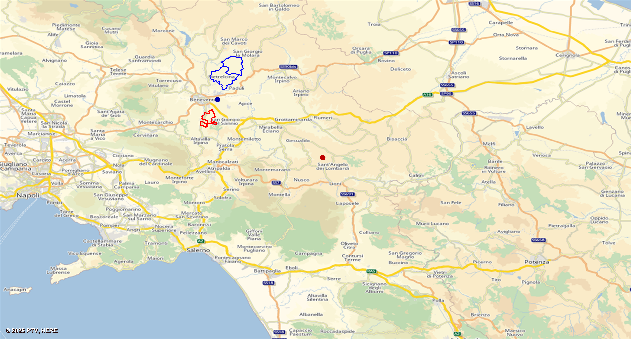
\includegraphics[width=1\textwidth]{images/1.png}}
    \caption{Redundancy map for Seismic Fault 1 – Low Intensity (8 km) - Destination}
\end{figure}

\begin{figure}[H]
\centering
{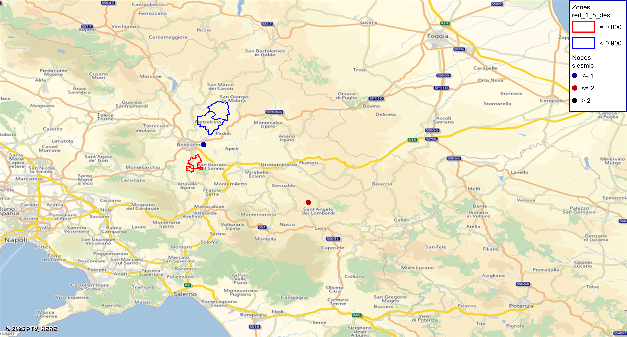
\includegraphics[width=1\textwidth]{images/2.png}}
    \caption{Redundancy map for Seismic Fault 1 – Low Intensity (8 km) - Origin}
\end{figure}


\begin{figure}[H]
\centering
{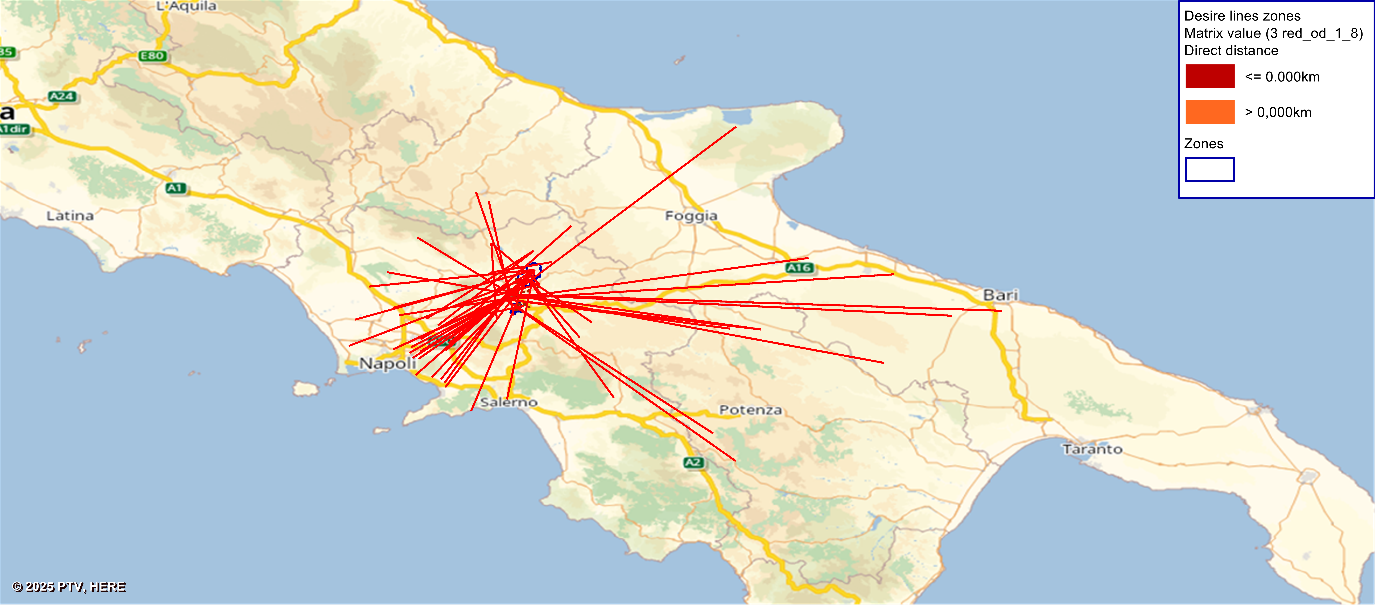
\includegraphics[width=1\textwidth]{images/3.png}}
    \caption{OD Pairs impacted from disruption for Seismic Fault 1}
\end{figure}

\begin{figure}[H]
\centering
{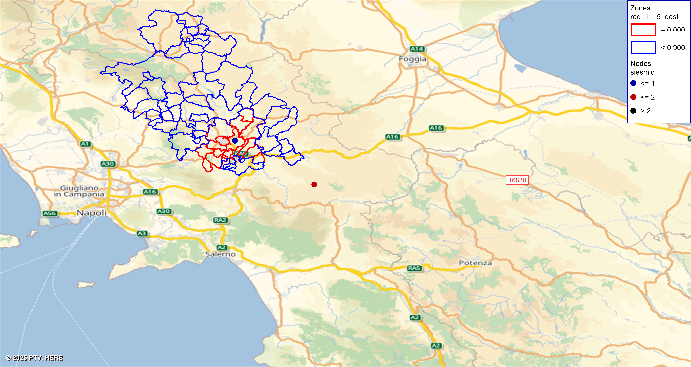
\includegraphics[width=1\textwidth]{images/4.png}}
    \caption{Redundancy map for Seismic Fault 1 – High Intensity (15 km) as Destination}
\end{figure}

\begin{figure}[H]
\centering
{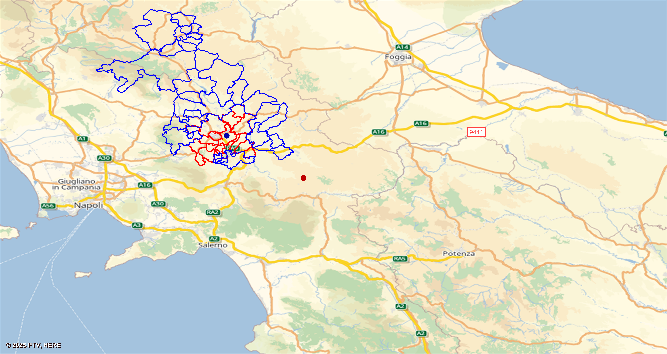
\includegraphics[width=1\textwidth]{images/5.png}}
    \caption{Redundancy map for Seismic Fault 1 – High Intensity (15 km) as Origin}
\end{figure}

\begin{figure}[H]
\centering
{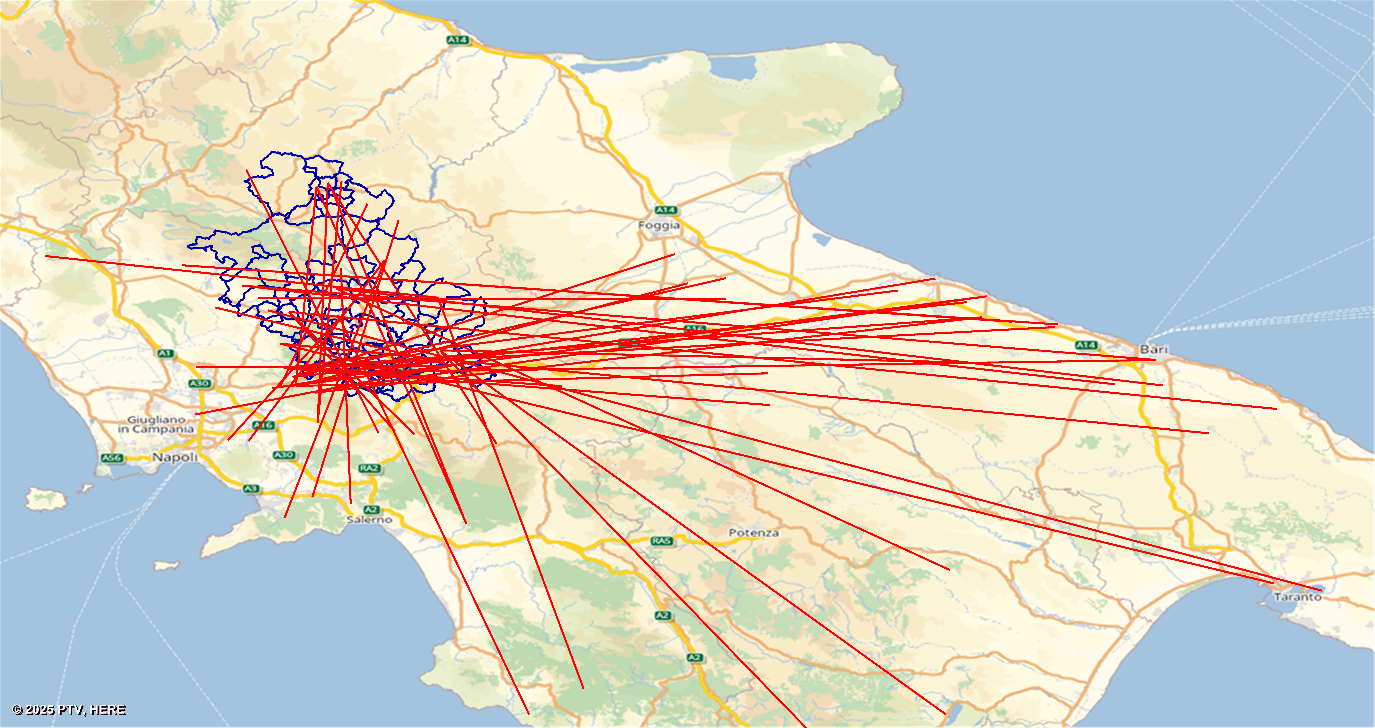
\includegraphics[width=1\textwidth]{images/6.png}}
    \caption{OD Pairs impacted from disruption for Seismic Fault 1(15 km)}
\end{figure}

\subsubsection{Seismic Fault 2}
\begin{itemize}
    \item \textbf{Low-Intensity (8 km radius)}
    \begin{itemize}
        \item No significantly affected zones were observed, indicating a more resilient network structure.
        \item OD pairs reflect a stable connectivity pattern with minor delays.
    \end{itemize}
    \item \textbf{High-Intensity (15 km radius)}
    \begin{itemize}
        \item A significant expansion of disconnected areas, with a clear increase in red zones.
        \item The number of impacted zones increased as more links failed, leading to widespread network fragmentation.
        \item OD pair analysis shows that zones impacted by severe seismic events extended eastward towards Apulia, specifically Bari province, due to limited major roads facilitating east-west connections (Figure D).
    \end{itemize}
\end{itemize}
Under low-intensity scenarios (8 km), the network remained largely intact, showing minimal impacts and no significant isolation.
However, high-intensity scenarios (15 km) had severe consequences, especially around Fault 1 (Benevento) and Fault 2 (Avellino).

Fault 1 scenarios showed the greatest damage, clearly isolating multiple zones—these appear as red zones on the redundancy maps.
Fault 2 had unexpected yet critical effects, extending disruptions significantly eastward towards Bari in Puglia. This impact is due to the limited number of major east-west routes, notably the critical A16 motorway, linking Campania to Puglia.

This eastward expansion of affected zones is due to the lower availability of major roads facilitating east-west connections in the region. When an earthquake occurs, the A16 motorway, which serves as a key east-west connection between Campania and Puglia, becomes severely impacted. Since this is one of the few major corridors linking the western and eastern parts of the region, its disruption leads to extensive accessibility losses. In contrast, Campania, especially Napoli province, has multiple access roads and a more integrated network, which allows it to maintain better connectivity even during disruptions.

\begin{figure}[H]
\centering
{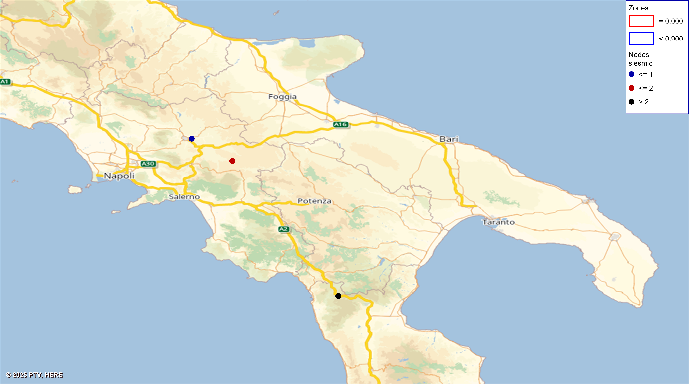
\includegraphics[width=1\textwidth]{images/7.png}}
    \caption{Redundancy map for Seismic Fault 2 – Low Intensity (8 km) as Destination}
\end{figure}

\begin{figure}[H]
\centering
{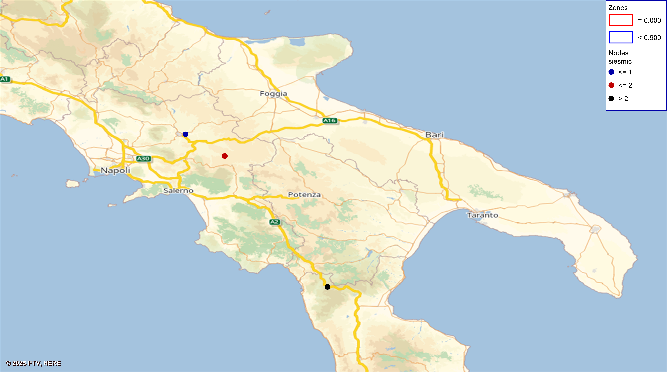
\includegraphics[width=1\textwidth]{images/8.png}}
    \caption{Redundancy map for Seismic Fault 2 – Low Intensity (8 km) as Origin}
\end{figure}

\begin{figure}[H]
\centering
{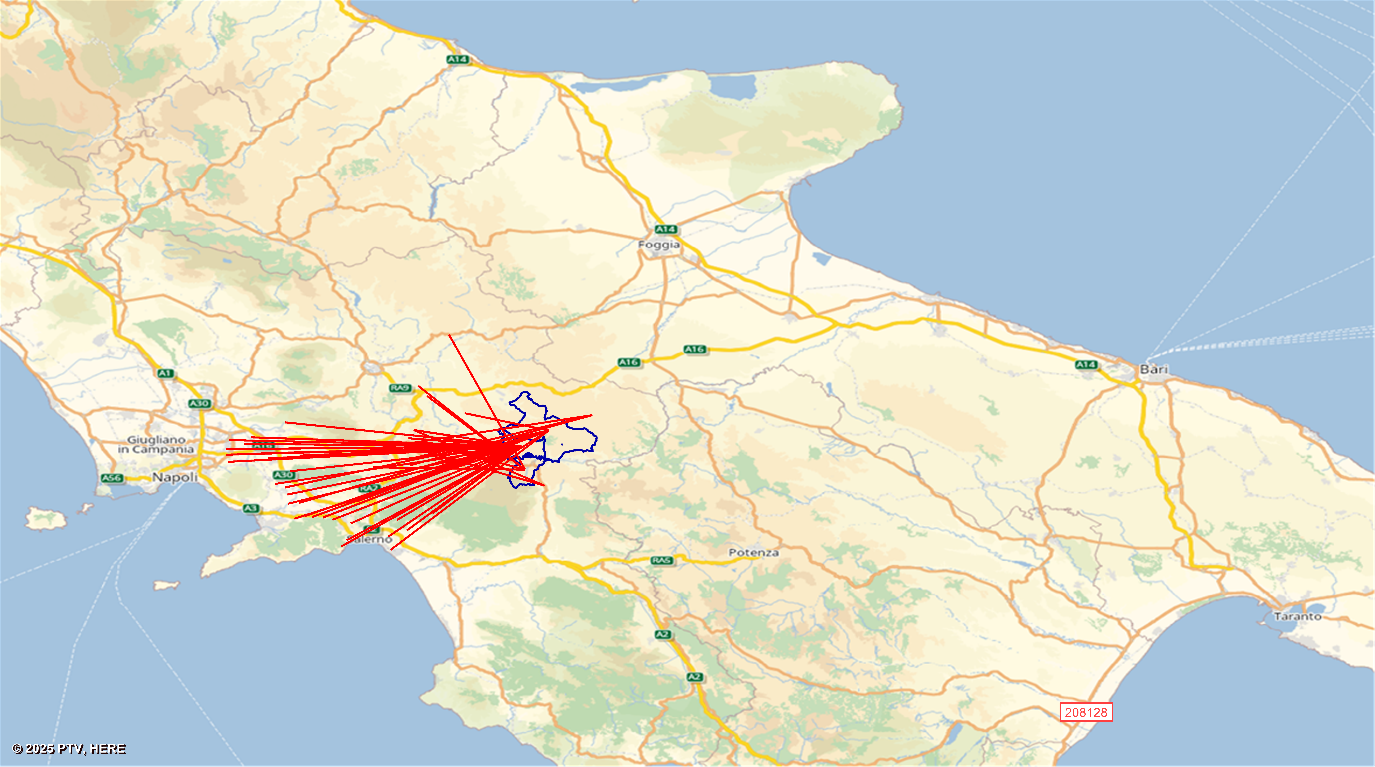
\includegraphics[width=1\textwidth]{images/9.png}}
    \caption{OD Pairs impacted from disruption for Seismic Fault 2 (8 km)}
\end{figure}

\begin{figure}[H]
\centering
{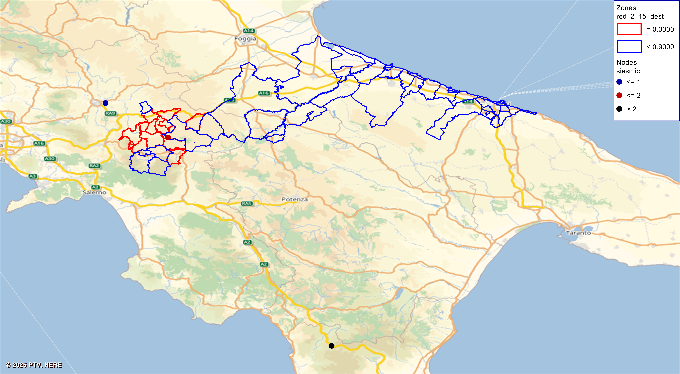
\includegraphics[width=1\textwidth]{images/10.png}}
    \caption{Redundancy map for Seismic Fault 2 – High Intensity (15 km) as Destination}
\end{figure}

\begin{figure}[H]
\centering
{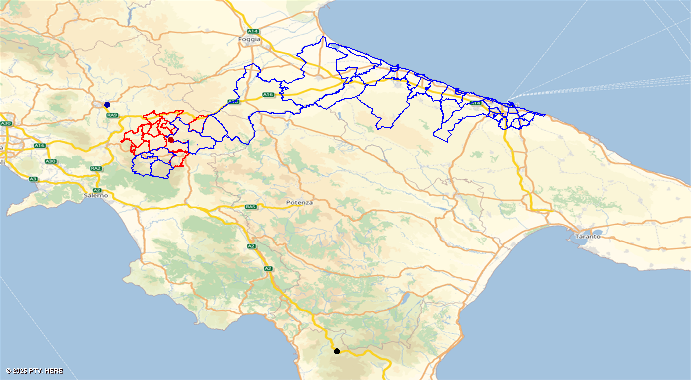
\includegraphics[width=1\textwidth]{images/11.png}}
    \caption{Redundancy map for Seismic Fault 2 – High Intensity (15 km) as Origin}
\end{figure}

\begin{figure}[H]
\centering
{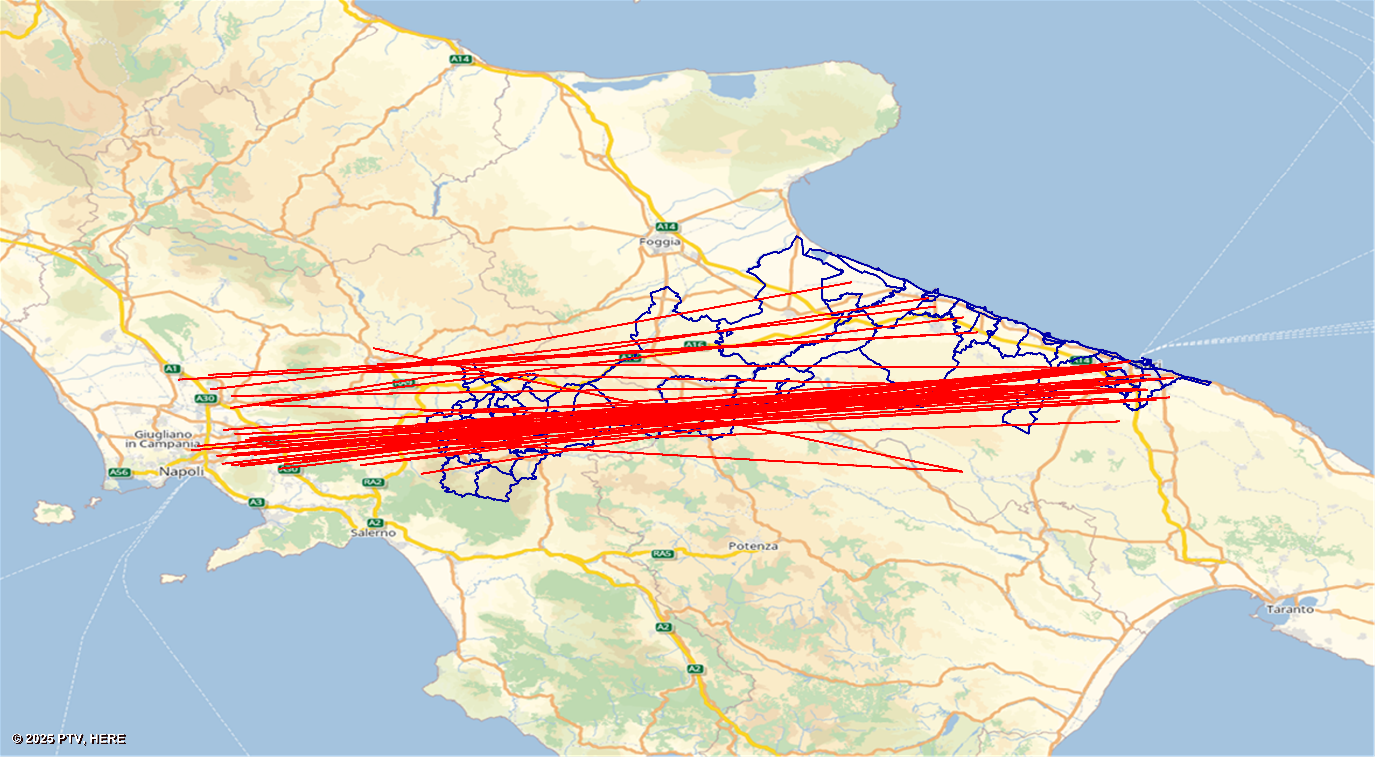
\includegraphics[width=1\textwidth]{images/12.png}}
    \caption{OD Pairs impacted from disruption for Seismic Fault 2 (15 km)}
\end{figure}

\subsubsection{Seismic Fault 3}
\begin{itemize}
    \item \textbf{Low-Intensity (8 km radius)}
    \begin{itemize}
        \item Limited impact on overall redundancy, with only a few zones experiencing travel time increases.
        \item OD pairs confirm that most connections remain intact.
    \end{itemize}
    
    \item \textbf{High-Intensity (15 km radius)}
    \begin{itemize}
        \item A substantial rise in disconnected zones, particularly in Calabria.
        \item The network was vulnerable due to fewer alternative routes and a lower node density.
        \item Although initially the least significant, Fault 3 became a critical scenario in high-intensity disruption, as the destruction of key nodes caused widespread connectivity loss in Calabria, reinforcing its vulnerability.
    \end{itemize}
\end{itemize}

\begin{figure}[H]
\centering
{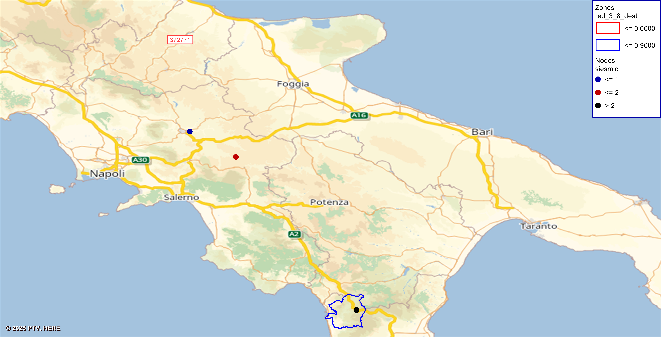
\includegraphics[width=1\textwidth]{images/13.png}}
    \caption{Redundancy map for Seismic Fault 3 – Low Intensity (8 km) as Destination}
\end{figure}

\begin{figure}[H]
\centering
{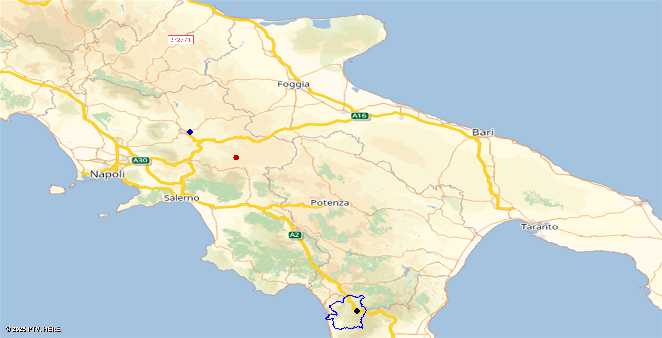
\includegraphics[width=1\textwidth]{images/14.png}}
    \caption{Redundancy map for Seismic Fault 3 – Low Intensity (8 km) as Origin}
\end{figure}

\begin{figure}[H]
\centering
{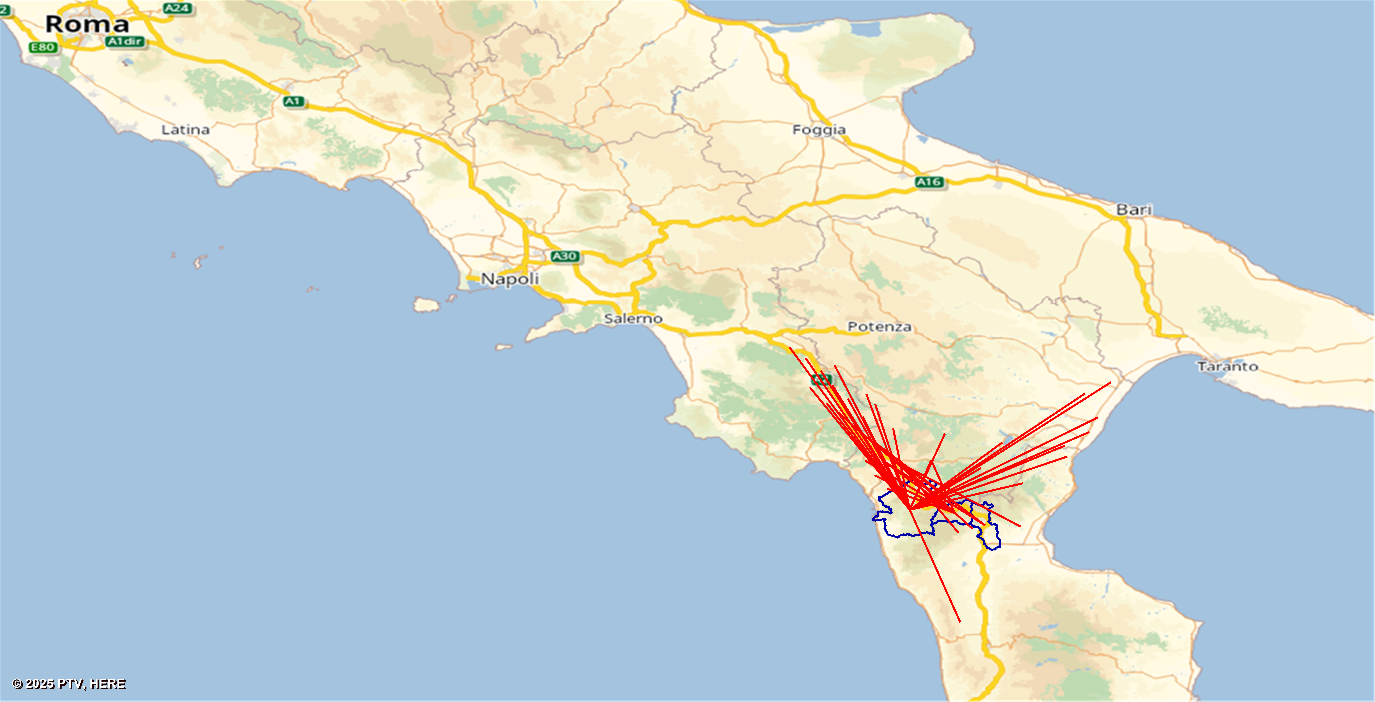
\includegraphics[width=1\textwidth]{images/15.png}}
    \caption{OD Pairs impacted from disruption for Seismic Fault 3 (8 km)}
\end{figure}

\begin{figure}[H]
\centering
{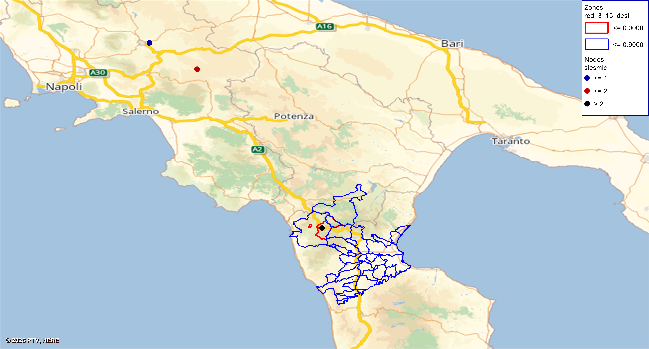
\includegraphics[width=1\textwidth]{images/16.png}}
    \caption{Redundancy map for Seismic Fault 3 – High Intensity (15 km) as Destination}
\end{figure}

\begin{figure}[H]
\centering
{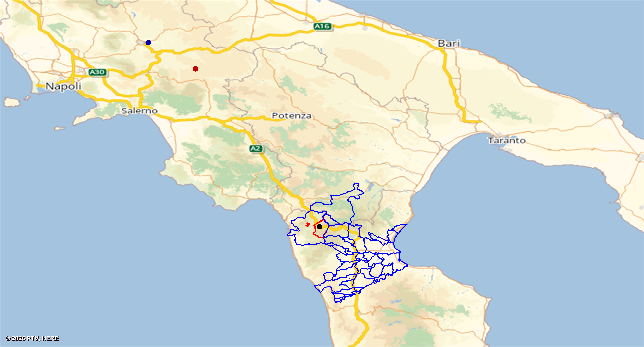
\includegraphics[width=1\textwidth]{images/17.png}}
    \caption{Redundancy map for Seismic Fault 3 – High Intensity (15 km) as Origin}
\end{figure}

\begin{figure}[H]
\centering
{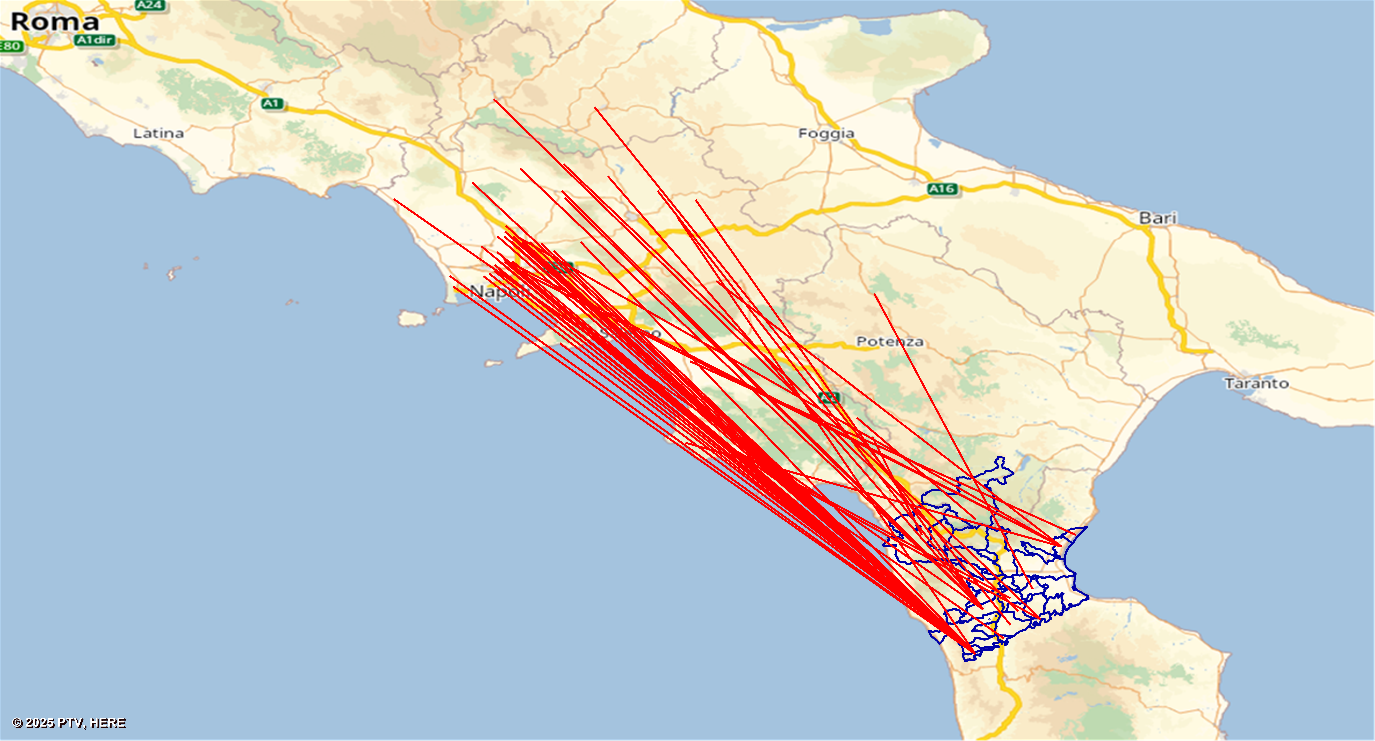
\includegraphics[width=1\textwidth]{images/18.png}}
    \caption{OD Pairs impacted from disruption for Seismic Fault 3 (15 km)}
\end{figure}

\subsection{Findings and Comparative Discussion}
\begin{itemize}
    \item \textbf{Seismic Fault 1} exhibited the most significant impact, particularly in high-intensity scenarios, where multiple red zones emerged, leading to complete disconnections.
    \item \textbf{Seismic Fault 2} displayed moderate effects, with connectivity still preserved in most scenarios, except for the high-intensity case, which caused noticeable disruptions, particularly affecting OD pairs between Campania and Puglia.
    \item \textbf{Seismic Fault 3}, despite being initially the least critical, became the most vulnerable in high-intensity scenarios due to its low node density. The loss of even a few crucial nodes led to widespread disconnections.
    \item \textbf{OD pairs} in high-intensity scenarios consistently showed lower redundancy values, signifying major delays and potential isolation of specific regions.
    \item \textbf{Motorways and major trunk roads} played a key role in maintaining connectivity, but disruptions forced detours onto secondary roads, leading to increased travel times.
\end{itemize}

\subsection{Implications for Seismic Resilience Planning}
\begin{itemize}
    \item \textbf{Highways and major roads} should be reinforced to mitigate cascading failures caused by disruptions.
    \item In \textbf{Benevento and Avellino} (Seismic Fault 2), particularly \textbf{Avellino}, redundancy strategies should be implemented, such as alternative expressways or reinforced detour routes, to minimize isolation risks.
    \item \textbf{Calabria} needs improved redundancy measures, as its low node density makes it highly susceptible to severe connectivity losses in extreme scenarios.
    \item \textbf{Emergency rerouting strategies} should focus on OD pairs with low redundancy values, ensuring minimal travel delays and maintaining regional accessibility.
\end{itemize}

\subsection{ Conclusion}
The redundancy analysis provides a clear picture of network vulnerability under seismic stress. While some regions exhibit greater resilience, others—such as Benevento and Avellino in the Faults 1 and 2 high-intensity scenario—face severe connectivity issues. The OD pair figures confirm the extent of network fragmentation, illustrating critical disconnections and major travel time increases, particularly in east-west transport corridors reliant on the A16 motorway.  By integrating redundancy insights into planning strategies, transport networks can be optimized to withstand future seismic disruptions, ensuring continued mobility and accessibility across Southern Italy.